% Esvil Protocol Whitepaper v2.0
% Asset-Agnostic RWA Tokenization on BNB Chain
\documentclass[11pt,a4paper]{article}

% Typography and fonts
\usepackage[T1]{fontenc}
\usepackage{mathpazo}
\usepackage{microtype}

% Layout
\usepackage[margin=1in]{geometry}
\usepackage{setspace}
\onehalfspacing

% Graphics and diagrams
\usepackage{graphicx}
\usepackage{tikz}
\usetikzlibrary{positioning, arrows.meta, shapes.geometric, fit, calc}

% Tables, lists, code
\usepackage{booktabs}
\usepackage{enumitem}
\usepackage{listings}
\usepackage{xcolor}
\usepackage{tabularx}
\usepackage{multirow}
\usepackage{array}
\usepackage{float}

% Caption styling
\usepackage{caption}
\captionsetup{
    font={small,sf},
    labelfont={bf},
    labelsep=period,
    justification=centering,
    margin=1cm
}
\usepackage[hidelinks]{hyperref}
\usepackage{url}

% Math
\usepackage{amsmath,amssymb,amsfonts}

% Section styling
\usepackage{titlesec}
\titleformat{\section}{\Large\bfseries}{\thesection.}{0.5em}{}
\titleformat{\subsection}{\large\bfseries}{\thesubsection}{0.5em}{}
\titleformat{\subsubsection}{\normalsize\bfseries}{\thesubsubsection}{0.5em}{}

% Header/Footer
\usepackage{fancyhdr}
\pagestyle{fancy}
\fancyhf{}
\fancyhead[L]{\small\textit{Esvil Protocol \textbar{} Whitepaper v2.0}}
\fancyhead[R]{\small\thepage}
\renewcommand{\headrulewidth}{0.4pt}

% Code listing style
\lstset{
    basicstyle=\ttfamily\small,
    breaklines=true,
    frame=single,
    backgroundcolor=\color{gray!5},
    keywordstyle=\color{blue!70!black},
    commentstyle=\color{green!50!black},
    stringstyle=\color{red!60!black},
    captionpos=b,
    tabsize=2,
}

% Custom colors (monochromatic brand palette)
\definecolor{esvilblack}{HTML}{1A1A1A}
\definecolor{esvilgray}{HTML}{4A4A4A}
\definecolor{esvildarkgray}{HTML}{2D2D2D}
\definecolor{esvillightgray}{HTML}{F5F5F5}

% Bibliography
\usepackage{natbib}

\begin{document}

% ============================================================
% TITLE PAGE
% ============================================================
\begin{titlepage}
\centering
\vspace*{2cm}

{\fontsize{14}{16}\selectfont\color{esvilblack}\textsc{Esvil Labs}}

\vspace{1.5cm}

{\fontsize{28}{34}\selectfont\bfseries\color{esvilblack} Esvil Protocol}

\vspace{0.5cm}

{\fontsize{14}{18}\selectfont\itshape An Asset-Agnostic, Compliance-Aware Framework\\for Real-World Asset Tokenization on BNB Chain}

\vspace{2cm}

{\large David Nzagha}\\[0.3cm]
{\normalsize Esvil Labs}

\vspace{1.5cm}

{\normalsize Version 2.0 \quad$\cdot$\quad February 2026}

\vspace{2cm}


\includegraphics[width=2.5cm]{figures/esvil-logo.png}

\vfill

{\small\textit{``Infrastructure for the ownership economy.\\Tokenizing the world's assets, one Diamond at a time.''}}

\vspace{1cm}
\end{titlepage}

% ============================================================
% ABSTRACT
% ============================================================
\newpage
\begin{abstract}
\noindent
The tokenization of real-world assets (RWAs) promises to unlock trillions of dollars in illiquid value, yet current protocols remain asset-specific, architecturally rigid, and poorly suited to evolving regulatory requirements. The \textbf{Esvil Protocol} introduces a decentralized, compliance-aware infrastructure for tokenizing \textit{any} real-world asset (including real estate, precious metals, commodities, intellectual property, and revenue-bearing instruments) on the BNB Chain. The protocol employs an \textbf{ERC-2535 Diamond Pattern} architecture, enabling modular, upgradeable smart contract systems where discrete functional facets (tokenization, compliance, trading, governance, revenue distribution) share a single proxy address and unified storage layer. A novel \textbf{E-RWA hybrid token standard} synthesizes ERC-3643 (T-REX compliant transfers), ERC-1643 (on-chain legal documents), ERC-1644 (controller-forced transfers), and ERC-1410 (partitioned balances into Class~A, B, and C tranches) to accommodate diverse asset classes under a single composable framework. Community governance through vote-escrowed \textbf{veESVL} tokens controls protocol parameters, asset approvals, verifier elections, and facet upgrades. A decentralized network of staked Asset Verifiers provides due diligence attestations, with slashing penalties ensuring accountability. We present the protocol's formal architecture, tokenization flow, cryptoeconomic model, governance mechanics, and regulatory compliance strategy across multiple jurisdictions.
\end{abstract}

\vspace{0.5cm}
\noindent\textbf{Keywords:} real-world assets, RWA tokenization, ERC-2535 Diamond, BNB Chain, compliance, decentralized governance, fractional ownership, DeFi

% ============================================================
% TABLE OF CONTENTS
% ============================================================
\newpage
\tableofcontents
\newpage

% ══════════════════════════════════════════════════════
\section{Introduction}
\label{sec:intro}

\subsection{Background}

Real-world assets, spanning real estate, precious metals, commodities, fine art, intellectual property, and private credit, represent an estimated \$900 trillion in global value~\cite{mckinsey2024}. The vast majority of this value remains illiquid, fractionally inaccessible, and confined within opaque, jurisdiction-bound markets. Blockchain-based tokenization offers a paradigm shift: representing ownership rights as programmable tokens that can be fractionalized, traded, and composed within decentralized financial systems~\cite{zetzsche2020, schar2021}.

Despite significant advances, the current RWA tokenization landscape suffers from three structural deficiencies:

\begin{enumerate}[nosep]
    \item \textbf{Asset Specificity:} Most protocols are purpose-built for a single asset class (real estate, gold, carbon credits), requiring entirely new infrastructure for each new category.
    \item \textbf{Architectural Rigidity:} Monolithic smart contract designs cannot adapt to evolving regulatory requirements, new asset types, or protocol improvements without costly redeployment.
    \item \textbf{Compliance Fragmentation:} Regulatory compliance is either absent (limiting institutional participation) or hardcoded (limiting jurisdictional flexibility), with no standard framework for composable compliance modules.
\end{enumerate}

\subsection{The Esvil Thesis}

The Esvil Protocol posits that RWA tokenization infrastructure should be \textit{asset-agnostic}: a single composable protocol capable of onboarding, verifying, tokenizing, trading, and distributing yield from any real-world asset, governed entirely by its community.

This asset-agnostic approach is enabled by three architectural innovations:

\begin{enumerate}[nosep]
    \item The \textbf{ERC-2535 Diamond Pattern}, which organizes protocol logic into modular, independently upgradeable facets behind a single proxy address.
    \item The \textbf{E-RWA hybrid token standard}, which synthesizes four ERC standards into a flexible container adaptable to any asset class.
    \item A \textbf{pluggable compliance engine} that enforces jurisdiction-specific rules through composable compliance modules, enabling the same protocol to operate across Nigeria, Switzerland, Estonia, Singapore, Liberland, Burkina Faso, and beyond.
\end{enumerate}

\subsection{Contributions}

This paper makes the following contributions:

\begin{enumerate}[nosep]
    \item A formal specification of the Diamond-based protocol architecture for asset-agnostic RWA tokenization (Section~\ref{sec:architecture}).
    \item The E-RWA hybrid token standard with multi-class partitioned ownership (Section~\ref{sec:erwa}).
    \item A complete tokenization flow from asset origination through verification, minting, distribution, and yield (Section~\ref{sec:flow}).
    \item Community governance mechanics with veESVL voting and decentralized verifier networks (Section~\ref{sec:governance}).
    \item Cryptoeconomic model with goal-oriented distribution and deflationary mechanics (Section~\ref{sec:tokenomics}).
    \item Multi-jurisdictional regulatory compliance strategy (Section~\ref{sec:compliance}).
\end{enumerate}

% ══════════════════════════════════════════════════════
\section{Related Work}
\label{sec:related}

The Esvil Protocol builds upon a rich body of work spanning blockchain architecture, asset tokenization, decentralized governance, MSME financial inclusion, and compliance-aware token standards. This section surveys the state of the art across seven domains, identifying both foundational contributions and the gaps that motivate Esvil's design.

\subsection{Blockchain Foundations and Smart Contract Platforms}

The conceptual foundation for decentralized, trustless systems was laid by Nakamoto~\cite{nakamoto2008}, whose Bitcoin whitepaper introduced the proof-of-work consensus mechanism and the notion of a distributed, immutable ledger. Buterin~\cite{buterin2014} extended this with Ethereum, introducing Turing-complete smart contracts that enabled programmable financial logic on-chain. Wood~\cite{wood2014} formalized Ethereum's execution model in the Yellow Paper, specifying the Ethereum Virtual Machine (EVM), gas mechanics, and state transition functions that underpin all ERC token standards used in the Esvil Protocol.

Benton and Radziwill~\cite{benton2017} provided an accessible primer for software quality professionals, disambiguating blockchain terminology and discussing practical utility beyond cryptocurrency, including supply chain provenance, digital identity, and certification. Their work underscored the importance of software quality assurance in blockchain deployments, a concern directly addressed by Esvil's multi-audit security model.

Szabo~\cite{szabo1997} anticipated many of these developments with his formalization of ``smart contracts'' as cryptographic protocols that embed contractual clauses into hardware and software. His vision of contracts that ``minimize the need for trusted intermediaries'' is central to Esvil's design philosophy: compliance, governance, and revenue distribution encoded entirely in on-chain logic.

\subsection{Asset Tokenization Frameworks}

The tokenization of real-world assets has attracted substantial academic and industry attention. Konashevych~\cite{konashevych2020} introduced the concept of ``Title Tokens'' for real estate, arguing for technological neutrality where blockchain-based registries coexist with traditional land registries. His framework illustrated how ownership tokens can be cryptographically linked to off-chain certificates (Figure~\ref{fig:konash-title}), addressing the legal, technological, and organizational dimensions of real estate tokenization. He established that tokenization is not merely a technical exercise but requires coordinated reform across property law, registry governance, and citizen rights. Esvil's DocumentFacet (ERC-1643) and multi-jurisdictional compliance strategy directly extend this vision to a broader asset universe.

\begin{figure}[H]
    \centering
    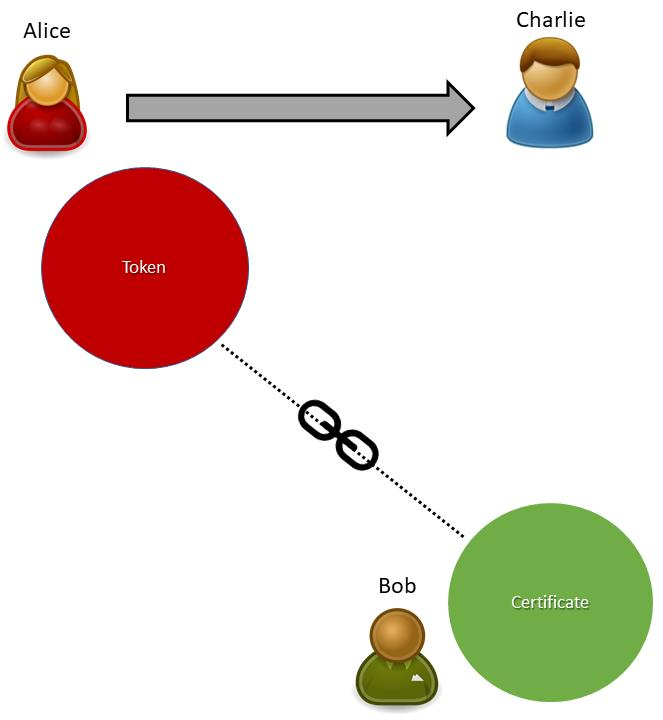
\includegraphics[width=0.55\textwidth]{figures/fig-konash-title-token.png}
    \caption{The Title Token model showing the cryptographic linkage between on-chain ownership tokens and off-chain certification authorities. Adapted from Konashevych~\cite{konashevych2020}.}
    \label{fig:konash-title}
\end{figure}

Joshi and Choudhury~\cite{joshi2022} proposed a blockchain-based framework for real estate tokenization using ERC-1155 tokens and IPFS for document storage. Their work identified the structural problems in traditional real estate markets (Figure~\ref{fig:joshi-problems}) and demonstrated that tokenization can lower entry barriers, fix liquidity constraints, and improve stakeholder interaction. However, their framework was limited to a single asset class (real estate) and a single token standard, lacking the multi-class partition model and compliance composability that Esvil provides through the E-RWA hybrid standard.

\begin{figure}[H]
    \centering
    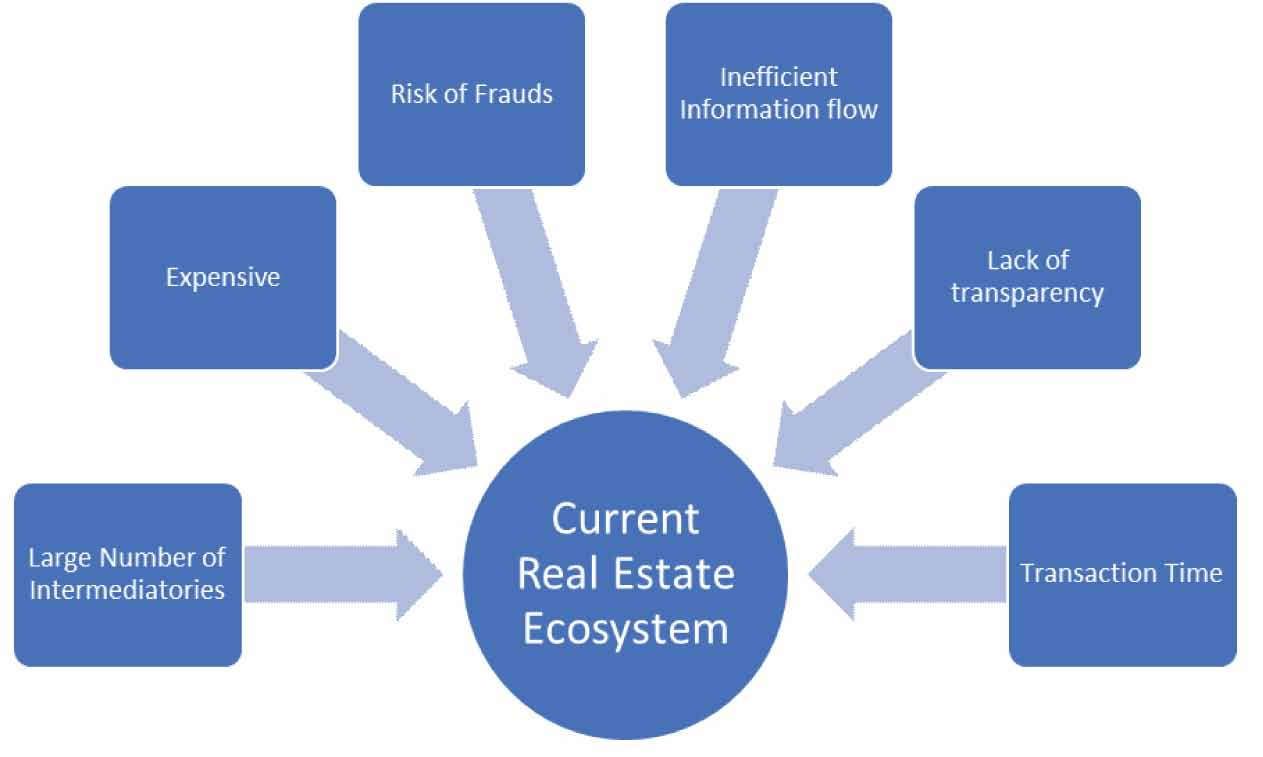
\includegraphics[width=0.85\textwidth]{figures/fig-joshi-re-problems.png}
    \caption{Structural problems in traditional real estate markets that tokenization aims to solve, including illiquidity, high entry barriers, and lack of transparency. Adapted from Joshi and Choudhury~\cite{joshi2022}.}
    \label{fig:joshi-problems}
\end{figure}

Juan et al.~\cite{juan2023} surveyed tokenized markets broadly, examining architectures, designs, challenges, and best practices for tokenized platforms across digital asset categories. Their taxonomy of tokenizable assets (Figure~\ref{fig:juan-taxonomy}) distinguishes between physical and digital assets, fungible and non-fungible representations, providing the conceptual foundation for Esvil's asset-agnostic approach. They identified four primary steps in tokenization (asset identification, valuation, parameterization, and smart contract creation) and highlighted cybersecurity threats and regulatory absence as key challenges. Esvil addresses both: the VerifierFacet provides decentralized valuation and due diligence, while the ComplianceFacet implements composable regulatory modules.

\begin{figure}[H]
    \centering
    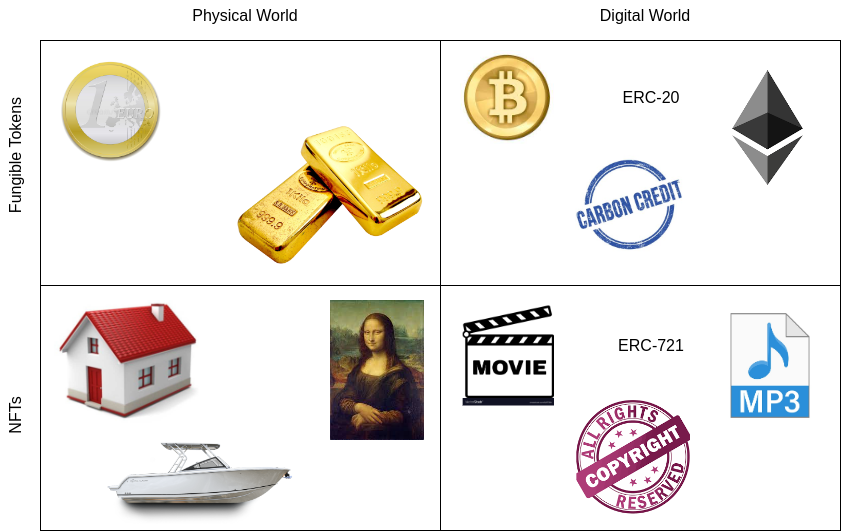
\includegraphics[width=0.75\textwidth]{figures/fig-juan-asset-taxonomy.png}
    \caption{Taxonomy of tokenizable assets across physical and digital categories, illustrating the breadth of asset classes that a tokenization protocol must accommodate. Adapted from Juan et al.~\cite{juan2023}.}
    \label{fig:juan-taxonomy}
\end{figure}

The OECD~\cite{oecd2022a} provided an institutional perspective on asset tokenization, analyzing how tokenization of financial instruments could improve market efficiency, reduce settlement times, and democratize access to investment products. Their report emphasized that regulatory clarity, investor protection, and interoperability standards are prerequisites for mainstream adoption, all of which inform Esvil's jurisdictional strategy and compliance architecture.

\subsection{Security Token Standards and Compliance}

The ERC-3643 (T-REX) standard~\cite{trex2021} established the paradigm for compliance-aware token transfers, introducing modular compliance agents that enforce transfer restrictions based on investor identity and jurisdictional rules. Edmonds et al.~\cite{edmonds2018} proposed the ERC-1400 family (ERC-1410 for partitioned balances, ERC-1643 for document management, ERC-1644 for controller operations), providing the primitives for representing complex security instruments on-chain. Esvil's E-RWA standard synthesizes all four of these standards into a single composable framework, an integration not previously achieved in any deployed protocol.

The Financial Cryptography and Data Security conference proceedings~\cite{baldimtsi2023} collected cutting-edge research on cryptographic protocols for financial systems, including work on privacy-preserving identity verification, DeFi liquidation mechanics, and formal security models for smart contracts. Esvil's zk-KYC integration draws from this body of work, employing zero-knowledge proofs for identity attestation without exposing personal data.

\subsection{Real-World Asset Identity and Authentication}

Norta, Udokwu, and Cra{\ss}~\cite{norta2024} addressed a critical gap in RWA tokenization: the authentication of real-world asset identities in blockchain-enabled inter-organizational systems. Their work combined a logistics DApp for RWA tracking with a multi-factor challenge-set self-sovereign identity authentication system (MFSSIA), using NFT-based identity attestations to prevent counterfeit circulation (Figure~\ref{fig:norta-mfssia}). Their configurable challenge-response framework for verifying asset authenticity across organizational boundaries directly informs Esvil's VerifierFacet design, where staked verifiers submit signed attestations after multi-dimensional due diligence (legal, physical, and valuation).

\begin{figure}[H]
    \centering
    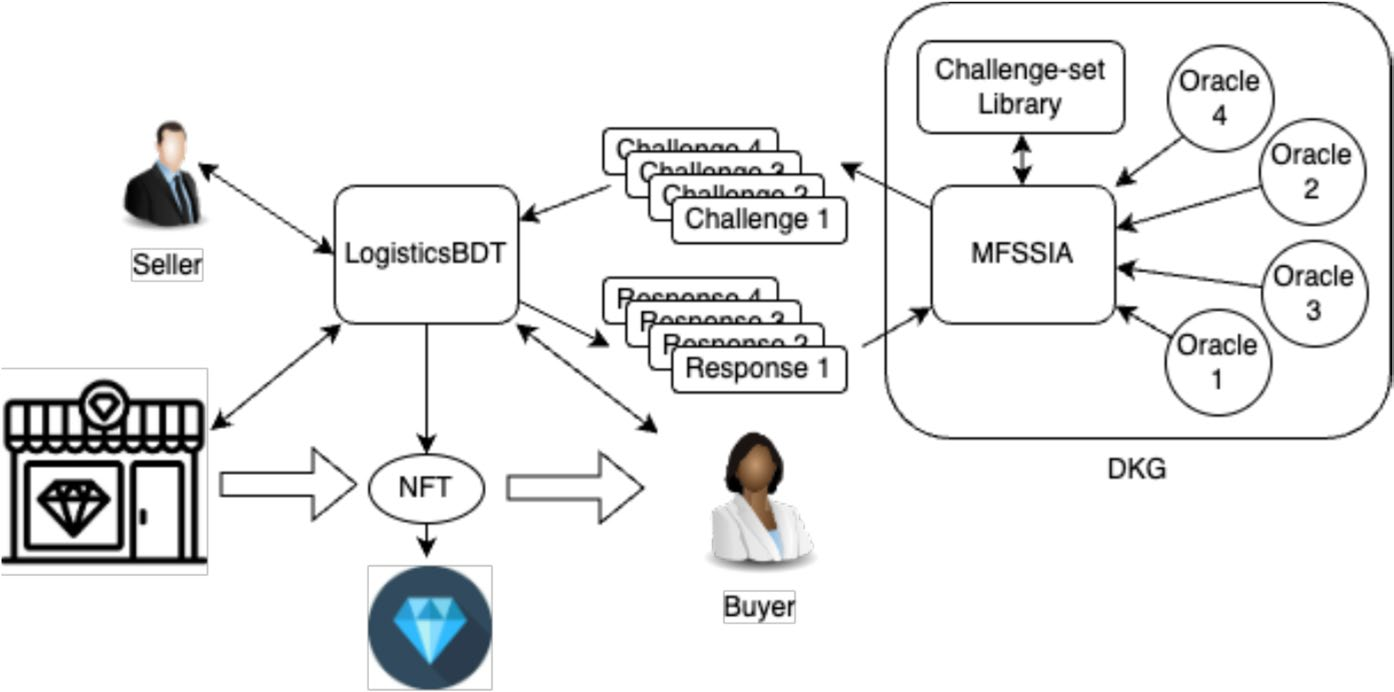
\includegraphics[width=0.85\textwidth]{figures/fig-norta-mfssia.png}
    \caption{The Multi-Factor Challenge-Set Self-Sovereign Identity Authentication (MFSSIA) system for real-world asset identity verification in blockchain-enabled inter-organizational systems. Adapted from Norta et al.~\cite{norta2024}.}
    \label{fig:norta-mfssia}
\end{figure}

Karamachoski, Marina, and Taskov~\cite{karamachoski2020} demonstrated blockchain-based certification management, applying Ethereum smart contracts to university diploma verification. While their application domain differs, the core architecture of on-chain certification with cryptographic hash verification and transparent auditability is directly applicable to Esvil's DocumentFacet, which anchors legal documents (title deeds, assay certificates, audit reports) on-chain via content hashes stored on IPFS/Arweave.

\subsection{Decentralized Finance and MSME Empowerment}

The role of MSMEs in emerging economies has been extensively documented. The OECD~\cite{oecd2022b} reported that SMEs account for over 90\% of businesses and 60-70\% of employment globally, yet face persistent barriers to finance, technology adoption, and market access. The World Bank~\cite{worldbank2023} highlighted that Africa's MSME sector, despite its dynamism, is severely constrained by capital access, with an estimated \$330 billion financing gap across the continent.

Amey Navarro~\cite{amey2024} investigated DeFi as a tool for MSME financial empowerment in Colombia, conducting expert interviews and MSME surveys to evaluate whether decentralized finance could address high interest rates, slow loan approvals, and limited access to capital. His findings confirmed DeFi's potential but identified knowledge gaps, regulatory uncertainty, and infrastructure limitations as barriers, challenges that Esvil addresses through its asset-agnostic tokenization framework, which enables MSMEs to unlock value from physical assets (commercial spaces, equipment, inventory) without relying on traditional banking infrastructure.

Riggs, Vyas, and Sethi~\cite{riggs2022} explored blockchain and Distributed Autonomous Community (DAC) ecosystems for democratizing finance and delivery of transport, housing, and urban infrastructure. Their work demonstrated how tokenized community assets could enable fractional ownership, transparent governance, and automated revenue distribution, a model closely aligned with Esvil's MSME physical spaces use case, where cooperatives co-own commercial spaces through E-RWA Class~B tokens.

Akaba, Norta, Udokwu, and Draheim~\cite{akaba2020} proposed a blockchain-based framework for e-procurement in Nigeria's public sector, addressing corruption, lack of transparency, and weak documentation systems. Their framework for on-chain interoperability, citizen participation, and project auditability provides relevant context for Esvil's deployment strategy in Nigeria, where regulatory compliance and institutional trust are critical adoption factors.

\subsection{Token Economics and Game Theory}

Udokwu~\cite{udokwu2024} formalized the token economics of a blockchain-based research collaboration platform using game theory, employing extensive-form games to analyze token distribution fairness and designing a logarithmic utility pricing model for token sustainability. His work demonstrated that self-sustaining token models require internal utility backing (not purely speculative value) and dynamic pricing mechanisms. Esvil's ESVL token economics incorporate these insights: the goal-oriented distribution model ties token emissions to protocol KPIs (Total Value Tokenized, active verifiers, governance participation), and the deflationary burn mechanics ensure long-term supply reduction.

Sch\"ar~\cite{schar2021} provided a comprehensive taxonomy of DeFi protocols, analyzing lending, decentralized exchanges, derivatives, and asset management on blockchain-based financial markets. His framework for understanding composability, the ability of DeFi protocols to interact and build upon each other, directly informs Esvil's Diamond Pattern architecture, where facets can be composed, upgraded, and extended without disrupting existing functionality.

Akbar et al.~\cite{akbar2025} designed and implemented a tokenized Decentralized Energy Management System (DEMS) for peer-to-peer energy trading, demonstrating how energy tokenization through custom tokens (ENRTokens) and smart contracts could automate trustless transactions. Their modular smart contract architecture (Figure~\ref{fig:dems-arch}) and microservices-based design for scalability across different hardware integrations parallel Esvil's facet-based modularity, though Esvil extends this pattern to arbitrary asset classes rather than a single commodity.

\begin{figure}[H]
    \centering
    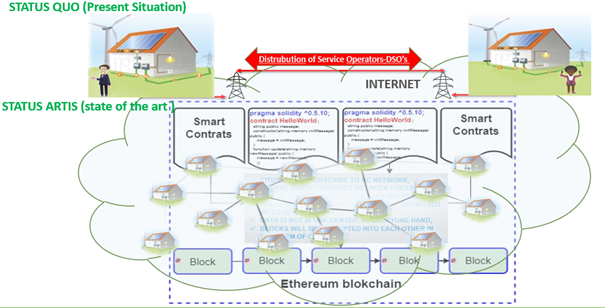
\includegraphics[width=0.85\textwidth]{figures/fig-dems-architecture.png}
    \caption{Architecture of the tokenized Decentralized Energy Management System (DEMS), illustrating modular smart contract design for peer-to-peer energy trading. Adapted from Akbar et al.~\cite{akbar2025}.}
    \label{fig:dems-arch}
\end{figure}

\subsection{Upgradeable Smart Contract Architecture}

The ERC-2535 Diamond standard~\cite{mudge2020} introduced a paradigm shift in smart contract architecture by enabling unlimited functionality through modular facets behind a single proxy address. Unlike earlier proxy patterns (transparent proxies, UUPS), the Diamond pattern supports granular function-level upgrades, shared storage across facets, and full on-chain introspection. While the Diamond pattern has been adopted in protocols like Aavegotchi and Louper, its application to RWA tokenization, where regulatory requirements demand frequent compliance module updates and new asset types require new functionality, has not been systematically explored prior to this work.

The combination of ERC-2535 with compliance-aware token standards (ERC-3643) and partitioned balances (ERC-1410) within a single Diamond represents a novel architectural contribution. Previous RWA protocols have employed monolithic contracts or loosely coupled multi-contract systems, both of which impose upgrade friction and composability costs that the Diamond pattern eliminates.

\subsection{Summary of Gaps}

Table~\ref{tab:gaps} summarizes the key limitations in existing work that the Esvil Protocol addresses.

\begin{table}[H]
\centering
\caption{Summary of gaps in existing work addressed by the Esvil Protocol.}
\label{tab:gaps}
\begin{tabularx}{\textwidth}{lXX}
\toprule
\textbf{Gap} & \textbf{Existing Approaches} & \textbf{Esvil's Solution} \\
\midrule
Asset specificity & Separate protocols per asset class (real estate, energy, gold) & Asset-agnostic E-RWA standard configurable for any asset \\
Architectural rigidity & Monolithic contracts or simple proxy patterns & ERC-2535 Diamond with modular, independently upgradeable facets \\
Compliance fragmentation & Hardcoded rules or absent compliance & Pluggable compliance modules composable per jurisdiction \\
MSME exclusion & Traditional finance barriers, high entry costs & Fractional tokenization, cooperative ownership models \\
Verification centralization & Centralized appraisers and auditors & Decentralized staked verifier network with slashing \\
Token sustainability & Speculative token models without utility backing & Goal-oriented distribution tied to protocol KPIs, deflationary burns \\
Identity privacy & KYC requiring full data disclosure & zk-KYC via ONCHAINID preserving user privacy \\
\bottomrule
\end{tabularx}
\end{table}

% ══════════════════════════════════════════════════════
\section{Protocol Architecture}
\label{sec:architecture}

\begin{figure}[H]
    \centering
    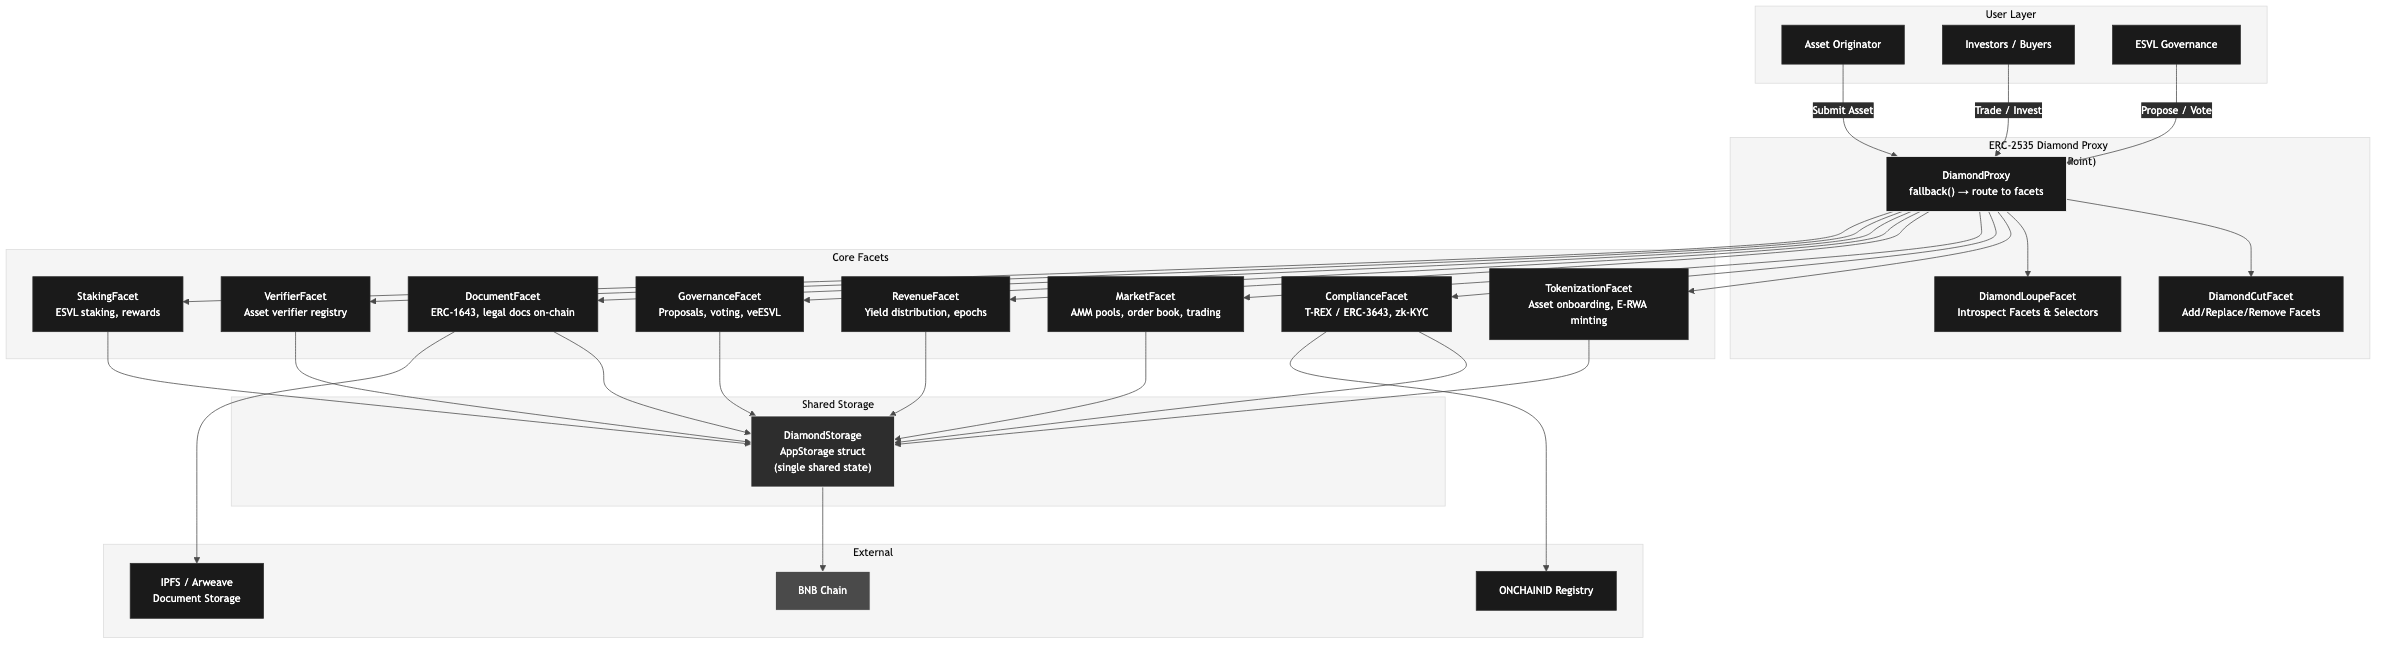
\includegraphics[width=\textwidth]{figures/architecture.png}
    \caption{Esvil Protocol architecture. The ERC-2535 Diamond Proxy routes all calls through a single address to modular facets (Tokenization, Compliance, Market, Revenue, Governance, Document, Verifier, Staking), all sharing a unified AppStorage struct. External integrations include BNB Chain, IPFS/Arweave for document storage, and the ONCHAINID registry for identity verification.}
    \label{fig:architecture}
\end{figure}

\subsection{Design Rationale: Why the Diamond Pattern}

Traditional smart contract systems deploy monolithic contracts or loosely coupled proxy-delegate patterns. Both approaches impose critical limitations for RWA tokenization:

\begin{itemize}[nosep]
    \item \textbf{Size limits:} The EVM's 24KB contract size limit constrains the amount of logic deployable in a single contract, forcing artificial splits.
    \item \textbf{Upgrade friction:} Transparent proxies and UUPS patterns require careful storage layout management and cannot add new state variables without migration risk.
    \item \textbf{Composability cost:} Multi-contract systems require cross-contract calls, increasing gas costs and attack surface.
\end{itemize}

The ERC-2535 Diamond standard~\cite{mudge2020} resolves these constraints by introducing \textit{facets}: independent contract modules whose functions are registered with a single Diamond proxy. The proxy's \texttt{fallback()} function routes calls to the appropriate facet based on function selector mappings.

\textbf{Key properties:}
\begin{itemize}[nosep]
    \item \textbf{No size limit:} The Diamond can incorporate unlimited functionality across unlimited facets.
    \item \textbf{Shared storage:} All facets read and write to a single \texttt{AppStorage} struct, eliminating cross-contract call overhead.
    \item \textbf{Granular upgrades:} Individual facets can be added, replaced, or removed without affecting others, through the \texttt{diamondCut()} function.
    \item \textbf{Single address:} Users and integrators interact with one contract address regardless of protocol complexity.
    \item \textbf{Introspection:} The \texttt{DiamondLoupeFacet} enables on-chain inspection of all registered facets and function selectors, ensuring full transparency.
\end{itemize}

\subsection{Facet Architecture}

The Esvil Diamond comprises eight core facets, two infrastructure facets, and a shared storage layer.

\subsubsection{Infrastructure Facets}

\begin{itemize}[nosep]
    \item \textbf{DiamondCutFacet:} Manages facet registration, replacement, and removal. Protected by governance timelock; only executable after successful veESVL vote and 48-hour delay.
    \item \textbf{DiamondLoupeFacet:} Implements ERC-2535 introspection interface. Returns all registered facets, their function selectors, and supported interfaces.
\end{itemize}

\subsubsection{Core Facets}

\begin{enumerate}[nosep]
    \item \textbf{TokenizationFacet:} Manages the asset onboarding pipeline. Receives verified asset metadata, mints E-RWA tokens with configurable partitions, and registers the asset in the global registry.

    \item \textbf{ComplianceFacet:} Enforces transfer restrictions based on jurisdiction, investor accreditation, and holding limits. Integrates with the ONCHAINID registry for zk-KYC verification. Implements composable compliance modules that can be swapped per jurisdiction.

    \item \textbf{MarketFacet:} Provides primary distribution (fixed-price offerings, Dutch auctions) and secondary market trading through integrated AMM pools. Manages liquidity provisioning and order matching.

    \item \textbf{RevenueFacet:} Collects and distributes yield from tokenized assets (rental income, commodity sales, royalties) to E-RWA holders on a pro-rata basis during defined revenue-sharing epochs.

    \item \textbf{GovernanceFacet:} Manages proposal submission, veESVL-weighted voting, quorum enforcement, timelock execution, and emergency actions. Controls all protocol parameter changes.

    \item \textbf{DocumentFacet:} Implements ERC-1643 for attaching, updating, and retrieving legal documents (title deeds, assay certificates, audit reports) linked to tokenized assets. Documents are stored on IPFS/Arweave with content hashes anchored on-chain.

    \item \textbf{VerifierFacet:} Manages the decentralized Asset Verifier network. Handles verifier applications, staking, assignment to assets, attestation submission, reputation tracking, and slashing.

    \item \textbf{StakingFacet:} Manages ESVL token staking for verifiers, governance participants, and liquidity providers. Handles reward distribution, unbonding periods, and slashing execution.
\end{enumerate}

\subsection{Shared Storage: AppStorage}

All facets share a single \texttt{AppStorage} struct via Solidity's diamond storage pattern. This eliminates storage collision risk and ensures atomic state transitions:

\begin{lstlisting}[caption={AppStorage struct (simplified)}]
struct AppStorage {
    // Asset Registry
    mapping(bytes32 => Asset) assets;
    mapping(bytes32 => TokenConfig) tokenConfigs;
    uint256 totalAssetsRegistered;

    // Compliance
    mapping(address => Identity) identities;
    mapping(bytes32 => ComplianceRule[]) jurisdictionRules;

    // Market
    mapping(bytes32 => Pool) liquidityPools;
    mapping(bytes32 => Offering) offerings;

    // Revenue
    mapping(bytes32 => Epoch[]) revenueEpochs;
    mapping(bytes32 => mapping(address => uint256)) claimable;

    // Governance
    mapping(uint256 => Proposal) proposals;
    mapping(address => VeLock) veLocks;
    uint256 proposalCount;

    // Verifiers
    mapping(address => Verifier) verifiers;
    mapping(bytes32 => Attestation[]) attestations;

    // Token
    IERC20 esvlToken;
    uint256 totalStaked;
}
\end{lstlisting}

\subsection{Upgrade Governance}

Protocol upgrades follow a strict governance pipeline:

\begin{enumerate}[nosep]
    \item A veESVL holder submits a proposal specifying the \texttt{diamondCut()} parameters (facet address, action, function selectors).
    \item The community votes over a 7-day period with a 10\% quorum requirement and 67\% approval threshold.
    \item Approved proposals enter a 48-hour timelock before execution.
    \item Emergency proposals (circuit breakers, critical patches) require 80\% supermajority and 24-hour timelock.
\end{enumerate}

This ensures that the protocol is both upgradeable and resistant to unilateral modification.

% ══════════════════════════════════════════════════════
\section{The E-RWA Hybrid Token Standard}
\label{sec:erwa}

\subsection{Design Philosophy}

The E-RWA token is a composable security token standard designed to represent ownership, access, and economic rights in any real-world asset. Rather than creating asset-specific token contracts, E-RWA provides a single, configurable token framework adaptable to diverse asset classes through parameterization.

\subsection{Standard Composition}

The E-RWA standard synthesizes four established ERC specifications:

\begin{table}[H]
\centering
\caption{ERC standards composing the E-RWA hybrid token.}
\label{tab:erc-composition}
\begin{tabularx}{\textwidth}{lX}
\toprule
\textbf{Standard} & \textbf{Function in E-RWA} \\
\midrule
ERC-3643 (T-REX) & Compliance-aware transfer restrictions, investor whitelisting, modular compliance agents \\
ERC-1643 & On-chain attachment of legal documents (deeds, certificates, audit reports) to token contracts \\
ERC-1644 & Controller-forced transfers for regulatory compliance, dispute resolution, and asset recovery \\
ERC-1410 & Partitioned balances enabling multiple token classes with distinct rights per asset \\
\bottomrule
\end{tabularx}
\end{table}

\subsection{Token Classes (Partitions)}

Each tokenized asset issues E-RWA tokens partitioned into three classes via ERC-1410:

\begin{table}[H]
\centering
\caption{E-RWA token class structure.}
\label{tab:token-classes}
\begin{tabularx}{\textwidth}{lXX}
\toprule
\textbf{Class} & \textbf{Rights} & \textbf{Transferability} \\
\midrule
A (Ownership) & Voting + revenue share + access rights & Restricted (KYC-gated, compliance-checked) \\
B (Access) & Revenue share + access/usage rights, no voting & Semi-restricted (lighter KYC) \\
C (Speculative) & Tradeable derivative, exposure to asset value & Free trading on AMM pools \\
\bottomrule
\end{tabularx}
\end{table}

This partition model accommodates diverse investor profiles within a single asset:
\begin{itemize}[nosep]
    \item Institutional investors acquire Class~A tokens for governance and yield.
    \item Retail participants purchase Class~B for passive income.
    \item Traders access Class~C for liquid exposure without compliance overhead.
\end{itemize}

\subsection{Asset Type Configurations}

The E-RWA framework adapts to different asset classes through configuration parameters:

\begin{table}[H]
\centering
\caption{E-RWA configuration by asset class.}
\label{tab:asset-configs}
\begin{tabularx}{\textwidth}{lXXX}
\toprule
\textbf{Asset Class} & \textbf{Yield Source} & \textbf{Valuation} & \textbf{Custody} \\
\midrule
Real Estate & Rental income & Appraised value & Title deed (ERC-1643) \\
Gold & None (appreciation) & Spot price oracle & Vault certificate \\
Commodities & Spot/futures spread & Market price & Warehouse receipt \\
IP / Royalties & Royalty streams & DCF model & License agreement \\
Private Credit & Interest payments & Face value & Loan agreement \\
\bottomrule
\end{tabularx}
\end{table}

\subsection{Formal Token Model}

Let $\mathcal{A}$ denote the set of tokenized assets. For each asset $a \in \mathcal{A}$, the E-RWA token system is defined as:

\begin{equation}
    T_a = (S_a, P_a, D_a, \Sigma_a)
\end{equation}

\noindent where $S_a = \{s^A_a, s^B_a, s^C_a\}$ is the supply across partitions, $P_a$ is the set of compliance predicates, $D_a$ is the document registry, and $\Sigma_a$ is the set of authorized signers (controller addresses).

A transfer of $n$ tokens of class $k$ from address $\alpha$ to $\beta$ is valid if and only if:

\begin{equation}
    \text{transfer}(a, k, \alpha, \beta, n) \Leftrightarrow \forall p \in P_a^k : p(\alpha, \beta, n) = 1
\end{equation}

\noindent where $P_a^k$ is the set of compliance predicates applicable to class $k$ of asset $a$. This formalization ensures that compliance is composable and asset-specific.

% ══════════════════════════════════════════════════════
\section{Tokenization Flow}
\label{sec:flow}

The tokenization lifecycle proceeds through four phases, each involving distinct protocol facets and participants (Figure~\ref{fig:tokenization-flow}).

\begin{figure}[H]
    \centering
    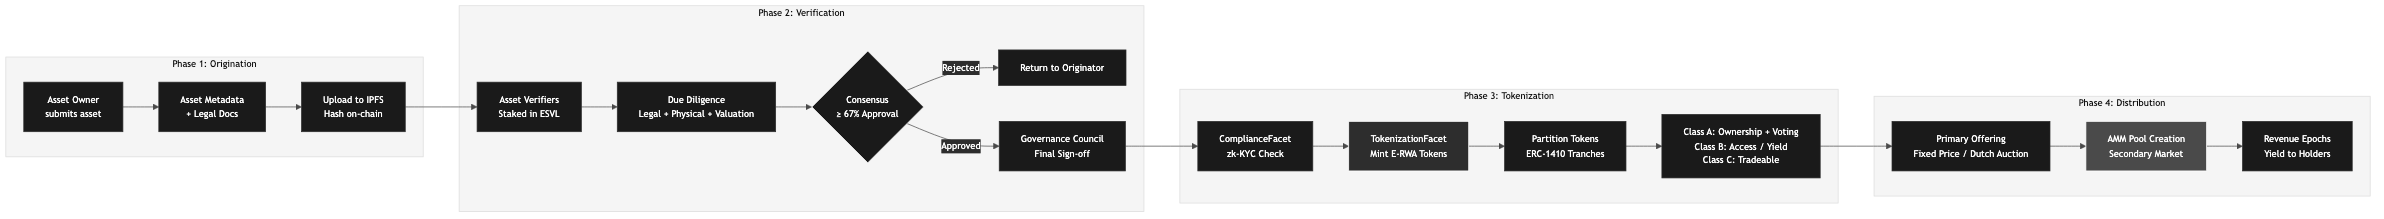
\includegraphics[width=\textwidth]{figures/tokenization-flow.png}
    \caption{End-to-end tokenization flow. An asset progresses through Origination (metadata and legal docs uploaded to IPFS), Verification (staked verifiers conduct due diligence, governance approves), Tokenization (compliance check, E-RWA minting with Class A/B/C partitions), and Distribution (primary offering followed by AMM secondary market and revenue epochs).}
    \label{fig:tokenization-flow}
\end{figure}

\subsection{Phase 1: Asset Origination}

An Asset Originator submits an asset for tokenization by providing:

\begin{enumerate}[nosep]
    \item \textbf{Asset metadata:} Type, description, location (if physical), valuation basis, and yield characteristics.
    \item \textbf{Legal documentation:} Title deeds, ownership certificates, assay reports, appraisals, or license agreements. Uploaded to IPFS/Arweave with content hashes stored on-chain via the DocumentFacet.
    \item \textbf{Tokenization parameters:} Requested total supply, class distribution (A/B/C ratios), target jurisdictions, and proposed compliance rules.
    \item \textbf{Origination bond:} A refundable ESVL deposit (minimum 10,000 ESVL) that is returned upon successful tokenization or forfeited if the asset fails verification due to fraud or misrepresentation.
\end{enumerate}

The DocumentFacet hashes and anchors all documents on-chain:

\begin{equation}
    D_a = \{(h_i, \text{uri}_i, t_i, \sigma_i)\}_{i=1}^{m}
\end{equation}

\noindent where $h_i = \text{keccak256}(\text{doc}_i)$, $\text{uri}_i$ is the IPFS/Arweave URI, $t_i$ is the timestamp, and $\sigma_i$ is the originator's signature.

\subsection{Phase 2: Verification}

The VerifierFacet assigns the asset to a panel of staked Asset Verifiers. The verification process comprises:

\begin{enumerate}[nosep]
    \item \textbf{Legal due diligence:} Verifying ownership records, encumbrances, and legal standing.
    \item \textbf{Physical inspection:} For physical assets (real estate, gold), on-site verification of existence, condition, and custody arrangements.
    \item \textbf{Valuation:} Independent appraisal aligned with the asset's valuation methodology.
    \item \textbf{Attestation:} Each verifier submits a signed attestation $A_v = (\text{assetId}, \text{verdict}, \text{findings}, \sigma_v)$ to the VerifierFacet.
\end{enumerate}

Consensus is reached when:

\begin{equation}
    \frac{\sum_{i=1}^{n} w_i \cdot C(v_i, a)}{\sum_{i=1}^{n} w_i} \geq Q_a
\end{equation}

\noindent where $w_i$ is the stake-weighted influence of verifier $v_i$, $C(v_i, a) \in \{0, 1\}$ is the verification verdict, and $Q_a \in [0.67, 0.75]$ is the asset-class-specific quorum threshold.

Upon consensus, the Governance Council (veESVL holders) performs a final sign-off vote before the asset proceeds to tokenization.

\subsection{Phase 3: Tokenization (Minting)}

The ComplianceFacet validates that the originator and proposed token structure comply with applicable jurisdictional rules. The TokenizationFacet then:

\begin{enumerate}[nosep]
    \item Creates the E-RWA token contract with configured partitions.
    \item Mints tokens according to the approved supply and class distribution.
    \item Registers the asset in the global registry within AppStorage.
    \item Links all verified documents via the DocumentFacet.
\end{enumerate}

\subsection{Phase 4: Distribution and Yield}

\subsubsection{Primary Distribution}

The MarketFacet supports two primary offering mechanisms:

\begin{itemize}[nosep]
    \item \textbf{Fixed-price offering:} Tokens sold at a predetermined price per unit, suitable for stable-value assets (real estate, bonds).
    \item \textbf{Dutch auction:} Price decreases from a ceiling until demand clears supply, suitable for assets with uncertain market pricing (art, rare commodities).
\end{itemize}

\subsubsection{Secondary Market}

After primary distribution, the MarketFacet creates AMM liquidity pools for Class~C tokens, enabling continuous trading and price discovery. Class~A and B tokens trade on a compliance-gated order book where both parties must satisfy the ComplianceFacet's transfer predicates.

\subsubsection{Revenue Distribution}

The RevenueFacet collects yield generated by tokenized assets and distributes it to E-RWA holders during defined epochs:

\begin{equation}
    r_{a,i} = R_a \cdot \frac{b_{a,i}}{\sum_{j} b_{a,j}}
\end{equation}

\noindent where $R_a$ is the total revenue collected for asset $a$ in the epoch, and $b_{a,i}$ is the token balance of holder $i$ (across eligible classes A and B).

% ══════════════════════════════════════════════════════
\section{Community Governance}
\label{sec:governance}

Esvil Protocol governance is fully community-driven, with no admin keys or centralized control after deployment. All protocol decisions flow through the GovernanceFacet (Figure~\ref{fig:governance}).

\begin{figure}[H]
    \centering
    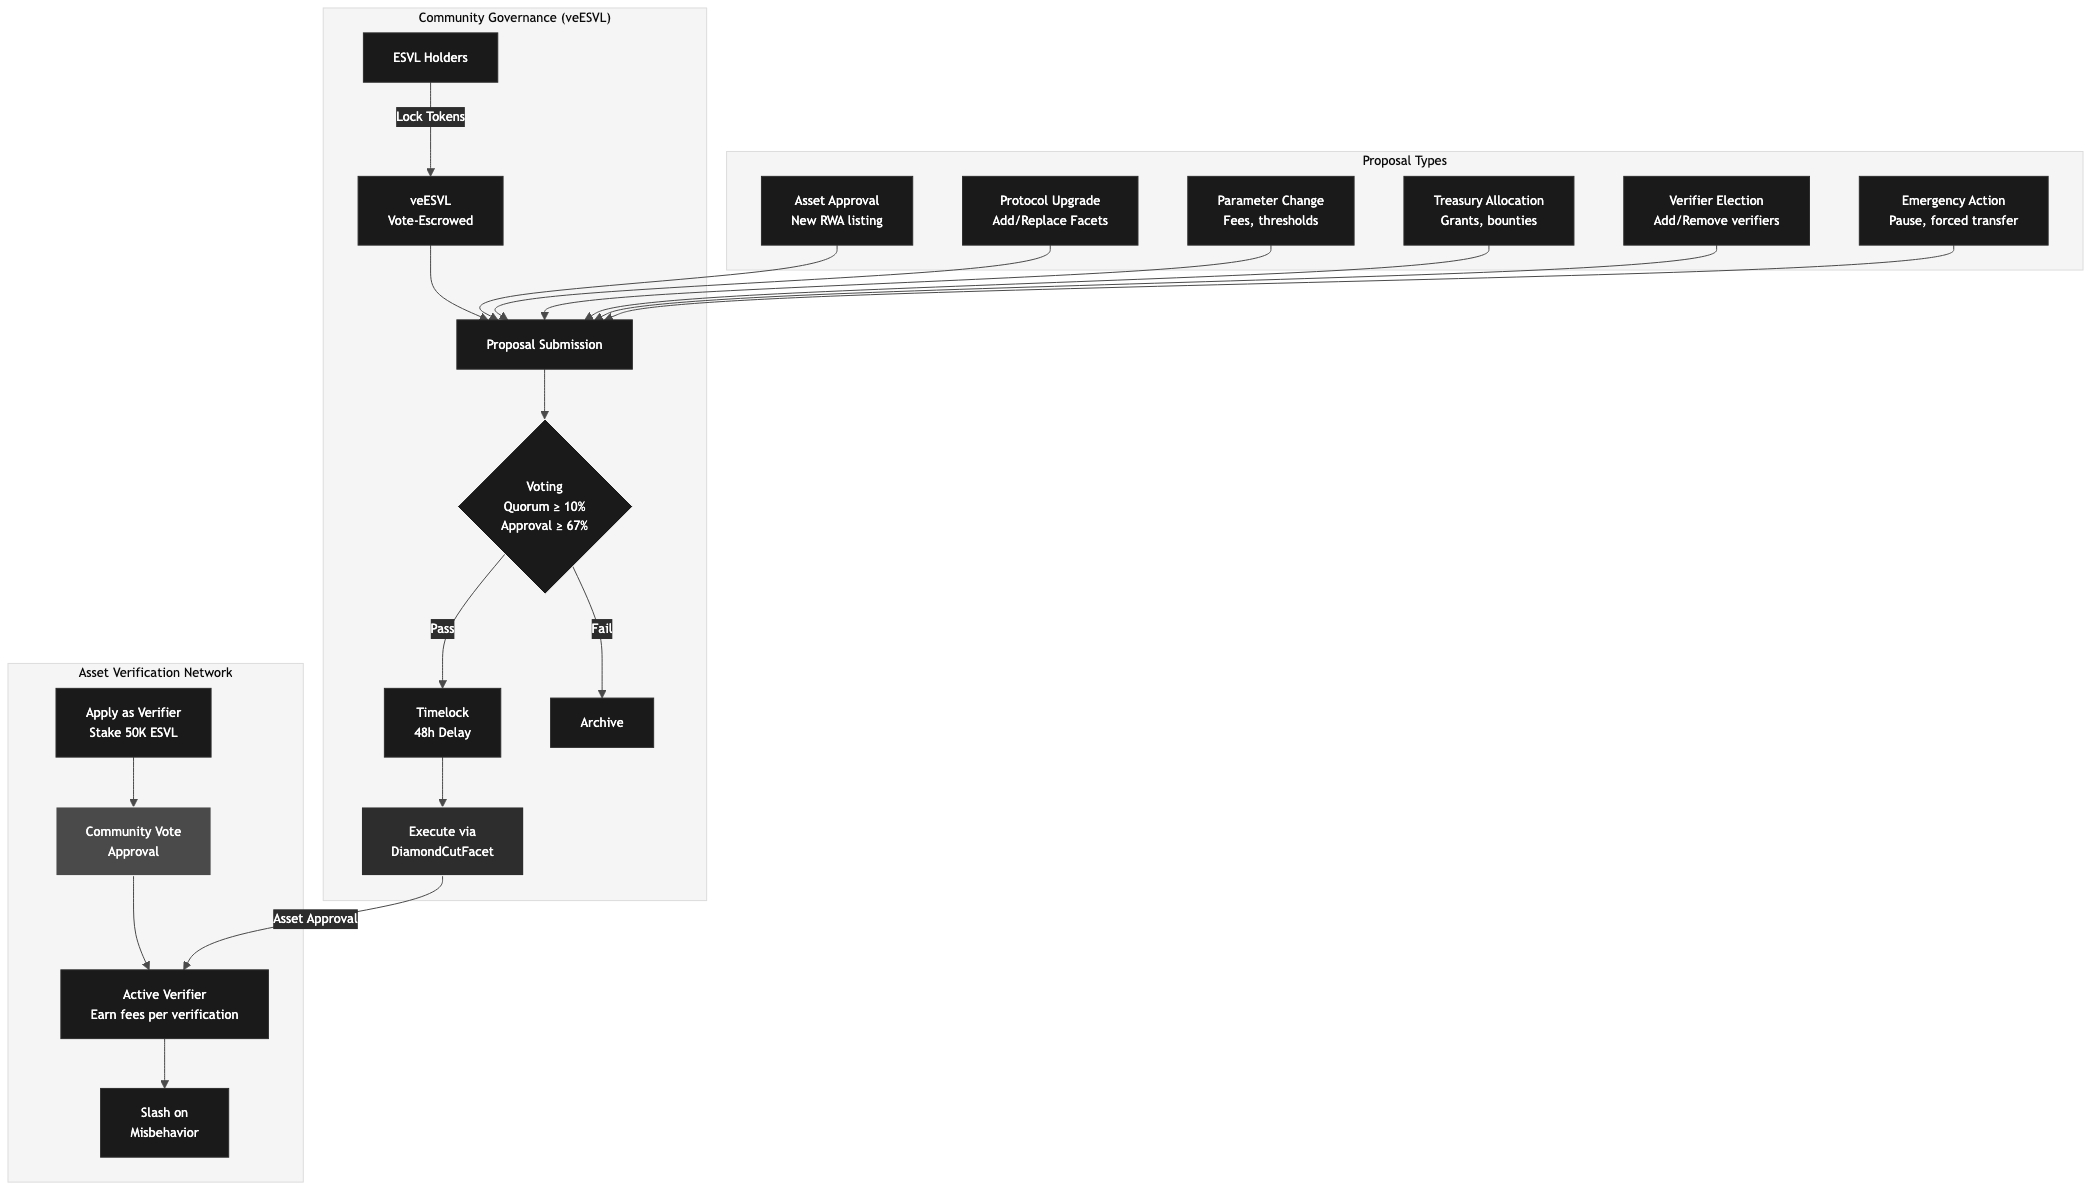
\includegraphics[width=\textwidth]{figures/governance.png}
    \caption{Governance and verification flow. ESVL holders lock tokens to obtain veESVL voting power. Six proposal types cover asset approvals, protocol upgrades, parameter changes, treasury allocation, verifier elections, and emergency actions. The Asset Verification Network operates through staked verifiers elected by community vote.}
    \label{fig:governance}
\end{figure}

\subsection{Vote-Escrowed ESVL (veESVL)}

Governance power is obtained by locking ESVL tokens for a chosen duration, receiving veESVL in return. Longer lock periods yield higher voting multipliers:

\begin{table}[H]
\centering
\caption{veESVL lock periods and voting multipliers.}
\label{tab:vesvl}
\begin{tabular}{lrr}
\toprule
\textbf{Lock Period} & \textbf{Multiplier} & \textbf{Decay} \\
\midrule
3 months & 1.0$\times$ & Linear \\
6 months & 1.5$\times$ & Linear \\
12 months & 2.5$\times$ & Linear \\
24 months & 5.0$\times$ & Linear \\
48 months & 10.0$\times$ & Linear \\
\bottomrule
\end{tabular}
\end{table}

veESVL voting power decays linearly toward the unlock date, incentivizing re-locking and long-term alignment:

\begin{equation}
    \text{veESVL}_i(t) = S_i \cdot m_i \cdot \frac{t_{\text{unlock}} - t}{t_{\text{unlock}} - t_{\text{lock}}}
\end{equation}

\noindent where $S_i$ is the locked amount, $m_i$ is the lock multiplier, and $t$ is the current time.

\subsection{Proposal Types}

Six categories of governance proposals are supported:

\begin{enumerate}[nosep]
    \item \textbf{Asset Approval:} Approve or reject a verified asset for tokenization.
    \item \textbf{Protocol Upgrade:} Add, replace, or remove Diamond facets via \texttt{diamondCut()}.
    \item \textbf{Parameter Change:} Adjust fees, quorum thresholds, slashing rates, epoch durations.
    \item \textbf{Treasury Allocation:} Deploy treasury funds for grants, bounties, or ecosystem development.
    \item \textbf{Verifier Election:} Add or remove Asset Verifiers from the active set.
    \item \textbf{Emergency Action:} Pause protocol, execute forced transfers (ERC-1644), or deploy critical patches.
\end{enumerate}

Standard proposals require 10\% quorum and 67\% approval. Emergency proposals require 5\% quorum and 80\% supermajority with a shortened 24-hour timelock.

\subsection{Decentralized Asset Verification Network}

Asset Verifiers are independent entities responsible for due diligence on proposed assets. The network operates as follows:

\begin{enumerate}[nosep]
    \item \textbf{Application:} Prospective verifiers stake a minimum of 50,000 ESVL and submit credentials.
    \item \textbf{Election:} veESVL holders vote to approve or reject the applicant.
    \item \textbf{Operation:} Active verifiers are assigned to asset verification panels, earning fees per completed verification.
    \item \textbf{Accountability:} Verifiers who submit fraudulent or negligent attestations face slashing penalties as defined in Table~\ref{tab:slashing}.
\end{enumerate}

\begin{table}[H]
\centering
\caption{Verifier slashing schedule.}
\label{tab:slashing}
\begin{tabular}{lr}
\toprule
\textbf{Offense} & \textbf{Slash} \\
\midrule
Negligent attestation (first) & 15\% of stake \\
Negligent attestation (repeat) & 35\% of stake \\
Fraudulent attestation & 100\% of stake + removal \\
Collusion with originator & 100\% + permanent ban \\
\bottomrule
\end{tabular}
\end{table}

Slashed tokens are burned permanently, creating deflationary pressure and deterring misbehavior.

% ══════════════════════════════════════════════════════
\section{Token Economics}
\label{sec:tokenomics}

The \textbf{ESVL} token is the native BEP-20 utility and governance token powering all protocol operations (Figure~\ref{fig:tokenomics}).

\begin{figure}[H]
    \centering
    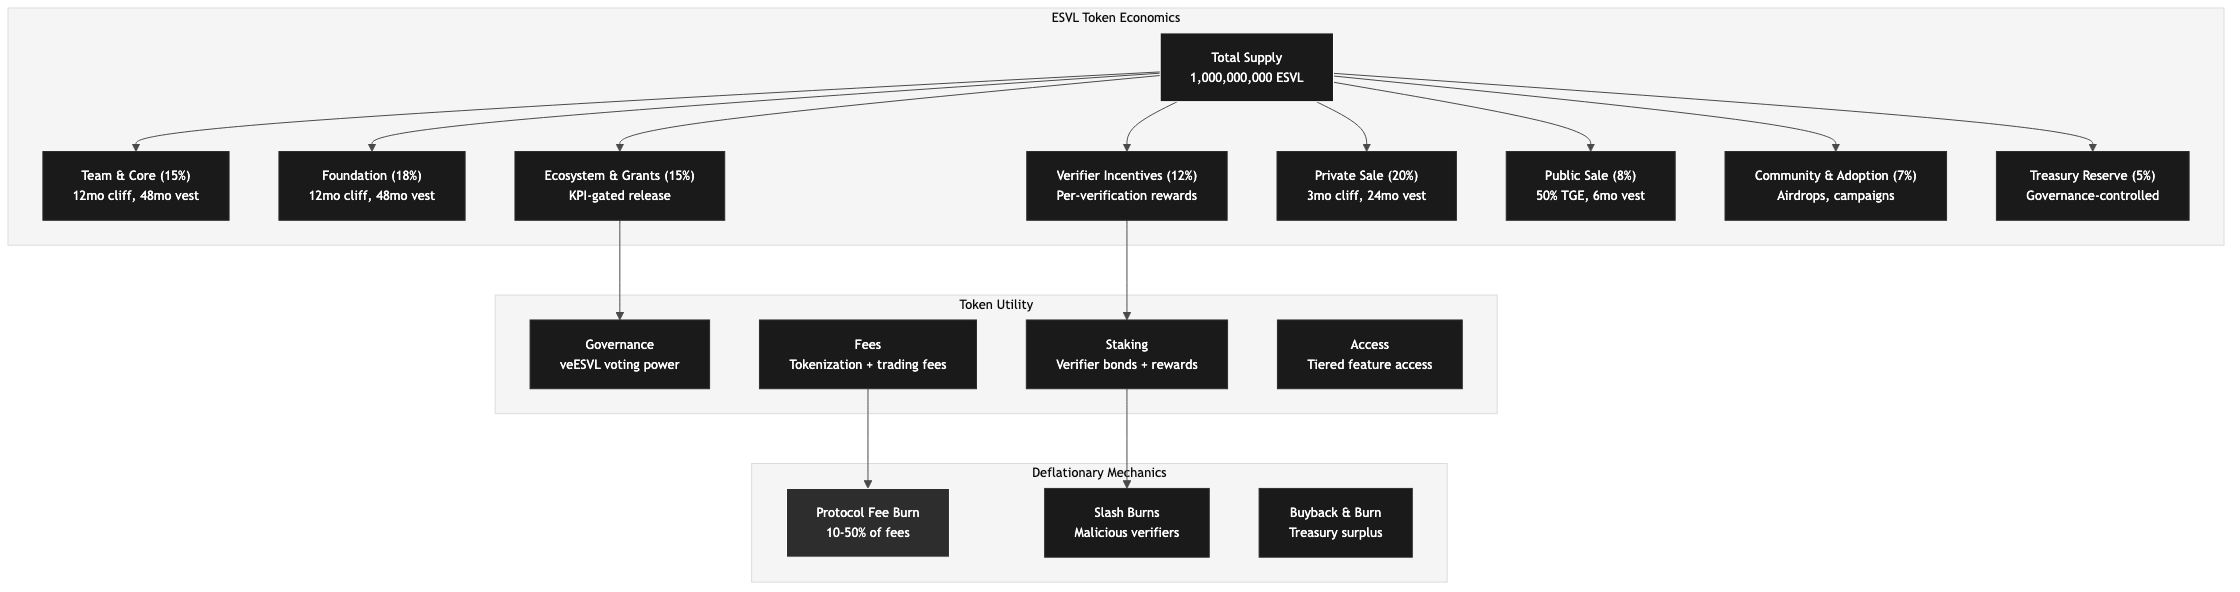
\includegraphics[width=\textwidth]{figures/tokenomics.png}
    \caption{ESVL token economics. Total supply of 1B tokens distributed across eight categories with vesting schedules. Token utility spans governance (veESVL), staking (verifier bonds), fees (tokenization and trading), and feature access. Deflationary mechanics include protocol fee burns, slash burns, and treasury buyback-and-burn programs.}
    \label{fig:tokenomics}
\end{figure}

\subsection{Token Utility}

\begin{table}[H]
\centering
\caption{ESVL token utility domains.}
\begin{tabularx}{\textwidth}{lX}
\toprule
\textbf{Domain} & \textbf{Function} \\
\midrule
Governance & Lock for veESVL, vote on all protocol decisions \\
Staking & Verifier bonds, liquidity incentives, protocol security \\
Fees & Tokenization fees, trading fees, verification fees (partial burn) \\
Access & Tiered feature access based on staked amount \\
Origination & Refundable bonds for asset submission \\
\bottomrule
\end{tabularx}
\end{table}

\subsection{Token Allocation}

Initial supply: 1,000,000,000 ESVL.

\begin{table}[H]
\centering
\caption{ESVL token allocation and vesting.}
\label{tab:allocation}
\begin{tabular}{lrrrr}
\toprule
\textbf{Category} & \textbf{\%} & \textbf{Cliff} & \textbf{Vest} & \textbf{TGE} \\
\midrule
Team \& Core & 15 & 12 mo & 48 mo & 0\% \\
Foundation & 18 & 12 mo & 48 mo & 0\% \\
Ecosystem \& Grants & 15 & 0 & 48 mo & -- \\
Verifier Incentives & 12 & 12 mo & 48 mo & 0\% \\
Private Sale & 20 & 3 mo & 24 mo & 10\% \\
Public Sale & 8 & 0 & 6 mo & 50\% \\
Community \& Adoption & 7 & 0 & 36 mo & 5\% \\
Treasury Reserve & 5 & -- & Gov. & 0\% \\
\bottomrule
\end{tabular}
\end{table}

\subsection{Goal-Oriented Distribution}

Ecosystem and Grant allocations follow a goal-oriented model where token emissions correlate with protocol performance. Let $\theta_t$ denote the current KPI state and $\theta^*_t$ the target:

\begin{equation}
    a_t = \rho(t, \theta_t) \cdot \Delta S_t
\end{equation}

\noindent where

\begin{equation}
    \rho(t, \theta_t) = \rho_m + (\rho_M - \rho_m) \cdot d(\theta_t, \theta^*_t)
\end{equation}

The composite distance function weights five KPIs:

\begin{table}[H]
\centering
\caption{KPI weights for goal-oriented distribution.}
\begin{tabular}{lr}
\toprule
\textbf{KPI} & \textbf{Weight} \\
\midrule
Total Value Tokenized (TVT) & 0.30 \\
Active Verifiers & 0.20 \\
Unique Token Holders & 0.20 \\
Trading Volume & 0.15 \\
Governance Participation & 0.15 \\
\bottomrule
\end{tabular}
\end{table}

\subsection{Deflationary Mechanics}

Three burning mechanisms counterbalance supply growth:

\begin{enumerate}[nosep]
    \item \textbf{Protocol fee burn:} A governance-adjustable percentage of all protocol fees is burned (10\% in Year~1, scaling to 50\% by Year~3).
    \item \textbf{Slash burns:} All slashed tokens from malicious verifiers are burned permanently.
    \item \textbf{Treasury buyback-and-burn:} When treasury reserves exceed 150\% of the target balance, surplus is used to buy and burn ESVL from the open market.
\end{enumerate}

Supply evolution follows:

\begin{equation}
    S_{t+1} = S_t + M_t - B_t^{\text{fee}} - B_t^{\text{slash}} - B_t^{\text{buyback}} - L_t + U_t
\end{equation}

\noindent where $M_t$ is minted tokens, $B_t$ terms are burns, and $L_t$, $U_t$ are governance-locked and unlocked tokens respectively.

\textbf{Proposition.} After all allocated tokens are minted ($M_t = 0$ for $t \geq \tau$), the expected supply change is negative, creating long-term deflationary pressure.

\textit{Proof.} For $t \geq \tau$:
\[
    \mathbb{E}[S_{t+1} - S_t] = -(B_t^{\text{fee}} + B_t^{\text{slash}} + B_t^{\text{buyback}}) - \mathbb{E}[L_t - U_t]
\]
All burn terms are positive, and assuming average governance locking exceeds unlocking ($\mathbb{E}[L_t] \geq \mathbb{E}[U_t]$), the expected supply change is strictly negative. \hfill$\square$

% ══════════════════════════════════════════════════════
\section{Regulatory Compliance}
\label{sec:compliance}

\subsection{Composable Compliance Modules}

The ComplianceFacet implements a pluggable compliance engine where jurisdiction-specific rules are encoded as modular compliance agents:

\begin{lstlisting}[caption={Compliance module interface}]
interface IComplianceModule {
    function canTransfer(
        address from,
        address to,
        uint256 amount,
        bytes32 partition
    ) external view returns (bool);

    function transferred(
        address from,
        address to,
        uint256 amount,
        bytes32 partition
    ) external;
}
\end{lstlisting}

Multiple compliance modules can be composed per asset. A transfer is valid only if \textit{all} applicable modules approve:

\begin{equation}
    \text{valid}(\alpha, \beta, n, k) = \bigwedge_{j=1}^{m} M_j.\text{canTransfer}(\alpha, \beta, n, k)
\end{equation}

\subsection{Supported Compliance Rules}

\begin{table}[H]
\centering
\caption{Example compliance module types.}
\begin{tabularx}{\textwidth}{lX}
\toprule
\textbf{Module} & \textbf{Rule} \\
\midrule
MaxHolders & Limits total number of token holders per asset \\
AccreditedOnly & Restricts Class~A to accredited/institutional investors \\
JurisdictionBlock & Blocks transfers to/from specified jurisdictions \\
HoldingPeriod & Enforces minimum holding periods before transfer \\
MaxOwnership & Caps maximum percentage ownership per holder \\
TransferWindow & Restricts transfers to defined time windows \\
\bottomrule
\end{tabularx}
\end{table}

\subsection{zk-KYC and ONCHAINID}

Identity verification uses privacy-preserving zero-knowledge proofs:

\begin{enumerate}[nosep]
    \item Users complete KYC with an authorized verification provider off-chain.
    \item The provider issues a zk-proof attesting to identity attributes (jurisdiction, accreditation status) without revealing personal data.
    \item The proof is registered in the ONCHAINID Registry, linked to the user's wallet.
    \item The ComplianceFacet queries ONCHAINID during transfer validation.
\end{enumerate}

This approach satisfies AML/KYC requirements while preserving user privacy, a critical consideration under GDPR and similar data protection frameworks.

\subsection{Jurisdictional Strategy}

\begin{table}[H]
\centering
\caption{Initial target jurisdictions and regulatory frameworks.}
\begin{tabularx}{\textwidth}{lXX}
\toprule
\textbf{Jurisdiction} & \textbf{Framework} & \textbf{Asset Focus} \\
\midrule
Nigeria & SEC Nigeria Digital Assets Rules & Real estate, commodities \\
Switzerland & DLT Act (2021) & Tokenized securities \\
Estonia & Virtual Asset Service Provider License & Digital asset custody \\
Singapore & MAS Payment Services Act & Tokenized funds \\
Dubai (DIFC) & DFSA Crypto Token Regime & Broad RWA coverage \\
Liberland & Liberland Blockchain Laws; LLM token framework & Tokenized governance, digital assets \\
Burkina Faso & Code Minier 2015 (revised); SONASP partnership model & Gold, mineral commodities \\
\bottomrule
\end{tabularx}
\end{table}

\subsubsection{Liberland: Blockchain-Native Sovereignty}

The Free Republic of Liberland presents a unique jurisdictional opportunity as a blockchain-native microstate. Liberland's governance infrastructure is built on distributed ledger technology, with its Liberland Merit (LLM) token serving as both a governance instrument and a unit of account. The state's legal framework explicitly recognizes tokenized assets and smart contract-based governance, making it one of the few jurisdictions where the Esvil Protocol's on-chain governance model (veESVL voting, Diamond upgrades, verifier elections) operates within a natively compatible legal environment. Liberland's openness to decentralized autonomous structures and its minimal regulatory overhead make it an ideal sandbox for pioneering novel RWA tokenization models before scaling to larger jurisdictions.

\subsubsection{Burkina Faso: Tokenized Gold and Local Economic Empowerment}

Burkina Faso is Africa's fourth-largest gold producer, with artisanal and small-scale mining (ASM) accounting for a significant share of national output. The \textit{Soci\'et\'e Nationale de Substances Pr\'ecieuses} (SONASP), the state agency responsible for purchasing, refining, and marketing artisanal gold, provides a natural institutional partner for tokenized gold provenance and trade. Under the revised \textit{Code Minier} (2015), Burkina Faso has progressively formalized its mining sector, creating regulatory pathways for technology-enabled traceability and value-chain transparency.

The Esvil Protocol's integration with Burkina Faso targets three objectives:

\begin{enumerate}[nosep]
    \item \textbf{Tokenized marked gold:} Artisanally mined gold, once assayed and marked by SONASP-accredited refineries, is tokenized as E-RWA tokens. The DocumentFacet anchors assay certificates, chain-of-custody records, and SONASP purchase receipts on-chain, creating an immutable provenance trail from mine site to market.
    \item \textbf{Local economic participation:} Gold miners and cooperatives receive Class~B E-RWA tokens representing fractional ownership in refined gold inventories, enabling them to participate in downstream value creation rather than selling raw output at discounted pit-head prices.
    \item \textbf{Sovereign gold reserves on-chain:} In partnership with SONASP, tokenized gold reserves can serve as collateral for decentralized lending, unlocking liquidity for local infrastructure development while maintaining sovereign custody of physical assets.
\end{enumerate}

This model directly addresses the value leakage that characterizes artisanal gold supply chains in West Africa, where intermediaries capture disproportionate margins. By tokenizing marked gold at the point of SONASP certification, the protocol ensures transparent pricing, reduces counterfeiting risk, and channels value back to producing communities.

% ══════════════════════════════════════════════════════
\section{Use Cases}
\label{sec:usecases}

\subsection{Real Estate: Fractional Commercial Ownership}

An office building valued at \$2M is tokenized into 2,000,000 E-RWA tokens. Class~A holders (accredited investors) vote on tenant selection and capital expenditures. Class~B holders receive monthly rental yield. Class~C tokens trade freely on the AMM, providing liquid exposure.

\subsection{Gold: Tokenized Vault Certificates}

A 100kg gold deposit in an audited vault is tokenized with each E-RWA token representing 0.001kg. DocumentFacet stores the vault certificate and quarterly audit reports. Verifiers include the vault operator and an independent auditor. No yield distribution; value tracks spot price via oracle integration.

\subsection{MSME Physical Spaces}

The protocol's original use case: MSMEs pool capital to co-own commercial spaces. 50 MSMEs each acquire Class~B tokens representing workspace access rights and pro-rata revenue from subleasing unused capacity. Governance (Class~A) is held by the community cooperative.

\subsection{Intellectual Property and Royalties}

A music catalog generating \$50K/month in streaming royalties is tokenized. Class~B holders receive monthly yield distributions through RevenueFacet epochs. The copyright holder retains Class~A governance rights over licensing decisions.

\subsection{Agricultural Commodities}

A 500-ton cocoa harvest in bonded warehouse is tokenized against warehouse receipts. DocumentFacet stores the receipt, quality certificates, and insurance documentation. Tokens are sold via Dutch auction, with delivery settlement coordinated off-chain through an authorized custodian.

\subsection{Burkina Faso: SONASP-Certified Artisanal Gold}

A cooperative of 200 artisanal miners in the Sahel region produces 50kg of gold per quarter. The gold is assayed, marked, and certified by a SONASP-accredited refinery. Each kilogram is tokenized into 1,000 E-RWA tokens with full provenance documentation (mine coordinates, assay report, SONASP receipt, chain-of-custody log) anchored via the DocumentFacet. Class~A governance is held by the cooperative's elected council. Class~B tokens distribute quarterly revenue from gold sales to member miners proportionally. Class~C tokens enable international investors to gain liquid exposure to Burkinab\`e artisanal gold at transparent, oracle-verified spot pricing, bypassing opaque intermediary networks.

% ══════════════════════════════════════════════════════
\section{Security and Risk Assessment}
\label{sec:security}

\subsection{Smart Contract Security}

\begin{itemize}[nosep]
    \item \textbf{Multiple audits:} Minimum three tier-1 audit firms before mainnet launch.
    \item \textbf{Formal verification:} Critical facets (Tokenization, Compliance, Governance) undergo formal verification.
    \item \textbf{Bug bounty:} Ongoing program with rewards up to \$500K for critical vulnerabilities.
    \item \textbf{Emergency pause:} GovernanceFacet includes circuit breaker functionality, activatable by supermajority vote.
    \item \textbf{Insurance fund:} 5\% of protocol revenue allocated to a smart contract cover fund.
\end{itemize}

\subsection{Diamond-Specific Risks}

\begin{table}[H]
\centering
\caption{Diamond pattern risk assessment.}
\begin{tabularx}{\textwidth}{lXll}
\toprule
\textbf{Risk} & \textbf{Description} & \textbf{Prob.} & \textbf{Mitigation} \\
\midrule
Selector clash & Two facets register the same function selector & Low & Automated clash detection in DiamondCutFacet \\
Storage collision & Facets overwrite shared storage slots & Low & Single AppStorage struct, no per-facet storage \\
Malicious upgrade & Governance compromised, bad facet deployed & Low & Timelock + multisig + supermajority requirement \\
Facet reentrancy & Cross-facet delegatecall reentrancy & Med & ReentrancyGuard in AppStorage, CEI pattern \\
\bottomrule
\end{tabularx}
\end{table}

\subsection{Economic Risk Matrix}

\begin{table}[H]
\centering
\caption{Protocol economic risk assessment.}
\begin{tabularx}{\textwidth}{lXll}
\toprule
\textbf{Category} & \textbf{Risk} & \textbf{Prob.} & \textbf{Impact} \\
\midrule
Verification & Verifier collusion or capture & Low & Critical \\
Market & Insufficient secondary market liquidity & Med & High \\
Economic & ESVL token price collapse & Med & Medium \\
Legal & Asset ownership disputed off-chain & Low & High \\
Adoption & Low originator demand & Med & High \\
Regulatory & Broad securities classification & Med & High \\
\bottomrule
\end{tabularx}
\end{table}

% ══════════════════════════════════════════════════════
\section{Implementation Roadmap}
\label{sec:roadmap}

\begin{table}[H]
\centering
\caption{Phased implementation roadmap.}
\begin{tabularx}{\textwidth}{lX}
\toprule
\textbf{Phase} & \textbf{Milestones} \\
\midrule
\textbf{Phase I} (Q2 2026) & Diamond proxy and core facets deployed to BNB Testnet; ESVL token contract; zk-KYC integration; governance voting \\
\textbf{Phase II} (Q3 2026) & First asset tokenized (real estate pilot, Nigeria); verifier network launched; DocumentFacet with IPFS \\
\textbf{Phase III} (Q4 2026) & AMM pools for Class~C tokens; revenue distribution epochs; second asset class (gold) \\
\textbf{Phase IV} (Q1 2027) & Mainnet launch on BNB Chain; multi-jurisdiction compliance modules; third asset class \\
\textbf{Phase V} (2027+) & Cross-chain bridges; institutional partnerships; additional jurisdictions; advanced financial products (collateralized positions, derivatives) \\
\bottomrule
\end{tabularx}
\end{table}

% ══════════════════════════════════════════════════════
\section{Conclusion}
\label{sec:conclusion}

The tokenization of real-world assets represents one of the most significant opportunities in decentralized finance, yet the infrastructure to support it at scale remains fragmented, rigid, and insufficiently compliant. The Esvil Protocol addresses these limitations through three architectural innovations: the ERC-2535 Diamond Pattern enables modular, upgradeable infrastructure behind a single contract address; the E-RWA hybrid token standard provides a composable framework adaptable to any asset class; and community governance through veESVL ensures that protocol evolution reflects the collective interests of its participants.

By making RWA tokenization asset-agnostic, compliance-aware, and community-governed, Esvil creates the conditions for a genuinely open market where real estate, precious metals, commodities, intellectual property, and any other value-bearing asset can be fractionalized, traded, and composed within a unified decentralized ecosystem on BNB Chain.

The protocol invites asset originators, verifiers, investors, developers, and governance participants to build the infrastructure that bridges traditional value and decentralized finance, one asset at a time.

% ══════════════════════════════════════════════════════
\bibliographystyle{plainnat}

\begin{thebibliography}{30}

\bibitem[Nakamoto(2008)]{nakamoto2008}
Nakamoto, S. (2008).
\newblock Bitcoin: A Peer-to-Peer Electronic Cash System.

\bibitem[Buterin(2014)]{buterin2014}
Buterin, V. (2014).
\newblock Ethereum: A Next-Generation Smart Contract and Decentralized Application Platform.
\newblock \textit{Ethereum Whitepaper}.

\bibitem[Wood(2014)]{wood2014}
Wood, G. (2014).
\newblock Ethereum: A Secure Decentralised Generalised Transaction Ledger.
\newblock \textit{Ethereum Yellow Paper}.

\bibitem[Mudge(2020)]{mudge2020}
Mudge, N. (2020).
\newblock ERC-2535: Diamonds, Multi-Facet Proxy.
\newblock \textit{Ethereum Improvement Proposals}.

\bibitem[T-REX(2021)]{trex2021}
T-REX Protocol (2021).
\newblock ERC-3643: T-REX Token for Real Estate Exchange.
\newblock \textit{Ethereum Improvement Proposals}.

\bibitem[Edmonds et~al.(2018)]{edmonds2018}
Edmonds, F., et al. (2018).
\newblock ERC-1400 Security Token Standard (ERC-1410, ERC-1643, ERC-1644).
\newblock \textit{Ethereum Improvement Proposals}.

\bibitem[Sch\"ar(2021)]{schar2021}
Sch\"ar, F. (2021).
\newblock Decentralized Finance: On Blockchain- and Smart Contract-Based Financial Markets.
\newblock \textit{Federal Reserve Bank of St.\ Louis Review}, 103(2):153--174.

\bibitem[Zetzsche et~al.(2020)]{zetzsche2020}
Zetzsche, D.\,A., Buckley, R.\,P., \& Arner, D.\,W. (2020).
\newblock Decentralized Finance (DeFi).
\newblock \textit{Journal of Financial Regulation}, 6(2):172--201.

\bibitem[McKinsey(2024)]{mckinsey2024}
McKinsey \& Company (2024).
\newblock Tokenization: A Digital Asset D\'ej\`a Vu.
\newblock \textit{McKinsey Global Institute Report}.

\bibitem[World Bank(2023)]{worldbank2023}
World Bank (2023).
\newblock Global Economic Prospects: Africa's Pulse.
\newblock \textit{World Bank Publications}.

\bibitem[IMF(2023)]{imf2023}
International Monetary Fund (2023).
\newblock World Economic Outlook: Navigating Global Divergences.
\newblock \textit{IMF Publications}.

\bibitem[OECD(2022a)]{oecd2022a}
OECD (2022).
\newblock Tokenisation of Assets and Financial Instruments.
\newblock \textit{OECD Publishing}.

\bibitem[OECD(2022b)]{oecd2022b}
OECD (2022).
\newblock SME and Entrepreneurship Outlook 2022.
\newblock \textit{OECD Publishing}.

\bibitem[OpenZeppelin(2024)]{openzeppelin2024}
OpenZeppelin (2024).
\newblock Contracts Documentation: Governor, ERC-20, Diamond Patterns.
\newblock \url{https://docs.openzeppelin.com/}.

\bibitem[Zyskind et~al.(2015)]{zyskind2015}
Zyskind, G., Nathan, O., \& Pentland, A. (2015).
\newblock Decentralizing Privacy: Using Blockchain to Protect Personal Data.
\newblock \textit{2015 IEEE Security and Privacy Workshops}, 180--184.

\bibitem[Lamport et~al.(1982)]{lamport1982}
Lamport, L., Shostak, R., \& Pease, M. (1982).
\newblock The Byzantine Generals Problem.
\newblock \textit{ACM TOPLAS}, 4(3):382--401.

\bibitem[BNB Chain(2024)]{bnbchain2024}
BNB Chain Documentation (2024).
\newblock BNB Smart Chain: Technical Overview and Developer Resources.
\newblock \url{https://docs.bnbchain.org/}.

\bibitem[Szabo(1997)]{szabo1997}
Szabo, N. (1997).
\newblock Formalizing and Securing Relationships on Public Networks.
\newblock \textit{First Monday}, 2(9).

\bibitem[Joshi and Choudhury(2022)]{joshi2022}
Joshi, S. \& Choudhury, A. (2022).
\newblock Tokenization of Real Estate Assets Using Blockchain.
\newblock \textit{International Journal of Intelligent Information Technologies}, 18(3):373--393.

\bibitem[Konashevych(2020)]{konashevych2020}
Konashevych, O. (2020).
\newblock General Concept of Real Estate Tokenization on Blockchain: The Right to Choose.
\newblock \textit{Preprint, Erasmus Mundus LAST-JD}. DOI:~10.13140/RG.2.2.33435.62244.

\bibitem[Juan et~al.(2023)]{juan2023}
Juan, A.\,A., Perez-Bernabeu, E., Li, Y., Martin, X.\,A., Ammouriova, M., \& Barrios, B.\,B. (2023).
\newblock Tokenized Markets Using Blockchain Technology: Exploring Recent Developments and Opportunities.
\newblock \textit{Information}, 14(6):347.

\bibitem[Norta et~al.(2024)]{norta2024}
Norta, A., Udokwu, C., \& Cra{\ss}, S. (2024).
\newblock Real-World Asset Identity Authentication in Blockchain Enabled Inter-Organizational Process-Aware Systems Involving Adjustable Challenge-Response Evaluation Sets.
\newblock \textit{SN Computer Science}, 5:936.

\bibitem[Karamachoski et~al.(2020)]{karamachoski2020}
Karamachoski, J., Marina, N., \& Taskov, P. (2020).
\newblock Blockchain-Based Application for Certification Management.
\newblock \textit{Tehnicki glasnik}, 14(4):488--492.

\bibitem[Amey Navarro(2024)]{amey2024}
Amey Navarro, L. (2024).
\newblock Decentralized Finance as a Tool for Financial Empowerment: A MSMEs Colombia Case Study.
\newblock \textit{Bachelor Thesis, Haute \'ecole de gestion de Gen\`eve (HEG-GE)}.

\bibitem[Riggs et~al.(2022)]{riggs2022}
Riggs, W., Vyas, V., \& Sethi, M. (2022).
\newblock Blockchain and Distributed Autonomous Community Ecosystems: Opportunities to Democratize Finance and Delivery of Transport, Housing, Urban Greening and Community Infrastructure.
\newblock \textit{Mineta Transportation Institute Publications}, Project 2165.

\bibitem[Akaba et~al.(2020)]{akaba2020}
Akaba, T.\,I., Norta, A., Udokwu, C., \& Draheim, D. (2020).
\newblock A Framework for the Adoption of Blockchain-Based e-Procurement Systems in the Public Sector: A Case Study of Nigeria.
\newblock In \textit{Responsible Design, Implementation and Use of ICT}, LNCS 12066, pp.~3--14. Springer.

\bibitem[Udokwu(2024)]{udokwu2024}
Udokwu, C. (2024).
\newblock Formalizing and Simulating the Token Aspects of Blockchain-Based Research Collaboration Platform Using Game Theory.
\newblock \textit{Mathematics}, 12(20):3252.

\bibitem[Akbar et~al.(2025)]{akbar2025}
Akbar, D., \"Unal, M., Akkaya, R., \& Balci, O. (2025).
\newblock Blockchain-Based Peer-to-Peer Energy Trading: Design and Implementation of the Tokenized Decentralized Energy Management System (DEMS).
\newblock \textit{Preprint}. DOI:~10.21203/rs.3.rs-6787257/v1.

\bibitem[Baldimtsi and Cachin(2023)]{baldimtsi2023}
Baldimtsi, F. \& Cachin, C., Eds. (2023).
\newblock \textit{Financial Cryptography and Data Security: 27th International Conference, FC 2023}.
\newblock LNCS 13950, Springer.

\bibitem[Benton and Radziwill(2017)]{benton2017}
Benton, M.\,C. \& Radziwill, N.\,M. (2017).
\newblock Quality and Innovation with Blockchain Technology.
\newblock \textit{arXiv preprint}, 1710.04130.

\end{thebibliography}

\end{document}
